\documentclass[varwidth=true, border=2pt]{standalone}
\usepackage{tikz}

\begin{document}
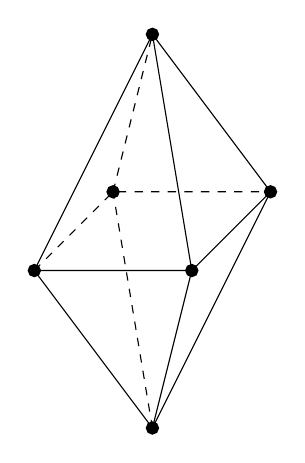
\begin{tikzpicture}
    \tikzstyle{point}=[circle,thick,draw=black,fill=black,inner sep=0pt,minimum width=4pt,minimum height=4pt]
    \node (a)[point] at (0,0) {};
    \node (b)[point] at (2,0) {};
    \node (c)[point] at (3,1) {};
    \node (d)[point] at (1,1) {};
    \node (e)[point] at (1.5,3) {};
    \node (f)[point] at (1.5,-2) {};
    \draw (a.center) -- (b.center) -- (c.center) -- (e.center) -- (b.center);
    \draw (a.center) -- (e.center);
    \draw[dashed] (a.center) -- (d.center) -- (c.center);
    \draw[dashed] (d.center) -- (e.center);

    \draw (a.center) -- (f.center) -- (b.center);
    \draw (f.center) -- (c.center);
    \draw[dashed] (f.center) -- (d.center);
\end{tikzpicture}
\end{document}
